\chapter{THIẾT KẾ PCB}
\section{Quá trình thiết kế PCB}
\textbf{Chuyển tất cả linh kiện từ Schematic qua PCB}
\begin{figure}[H]
    \centering
    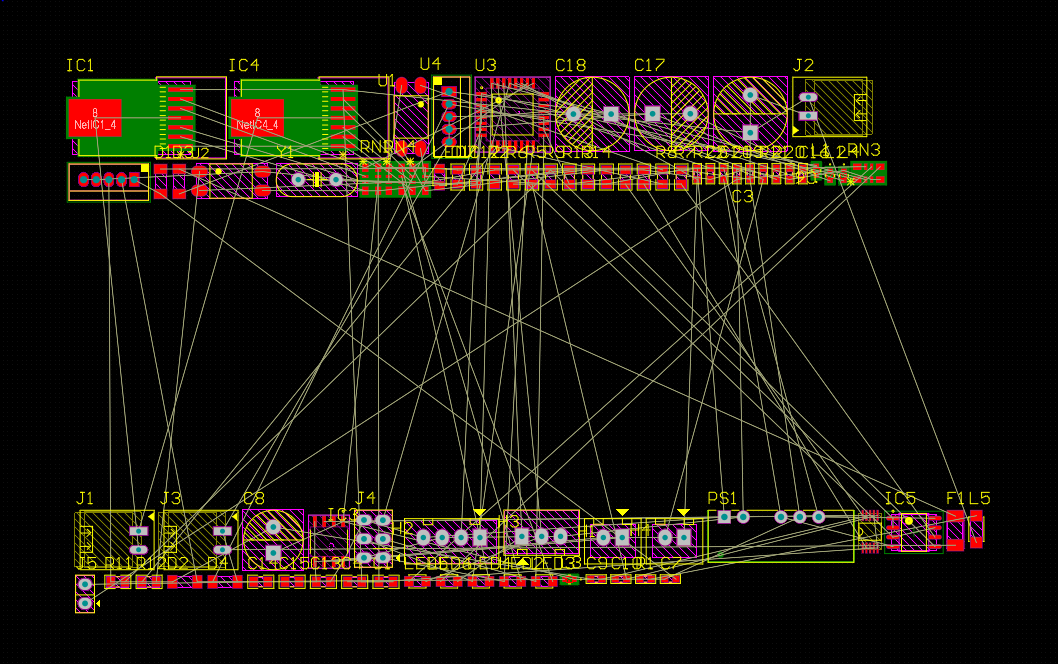
\includegraphics[width=1\textwidth]{pictures/7a.png}
\end{figure}
\begin{figure}[H]
    \centering
    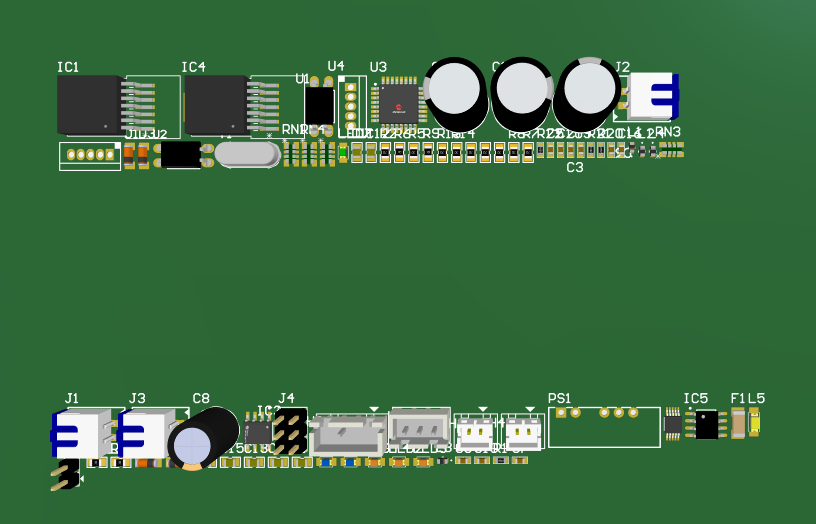
\includegraphics[width=1\textwidth]{pictures/7b.png}
\end{figure}
Ở bước này cần kiểm tra nếu có linh kiện nào không chuyển được qua PCB hay gặp các lỗi thiếu footprint như bên dưới thì cần kiểm tra lại Schematic.
\begin{figure}[H]
    \centering
    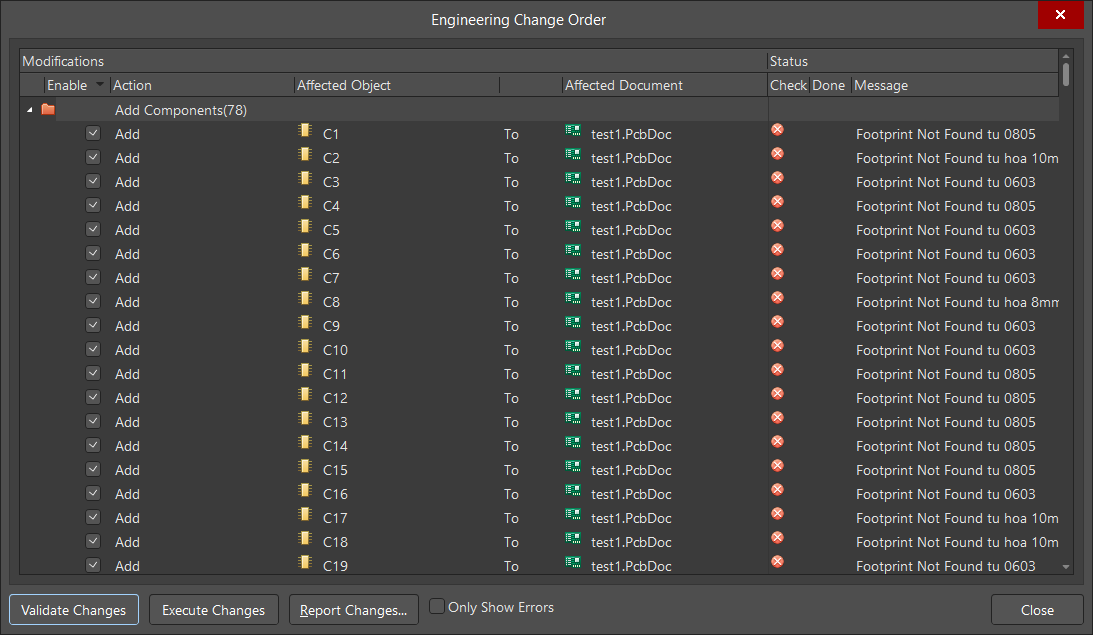
\includegraphics[width=1\textwidth]{pictures/7c.png}
\end{figure}
\cleardoublepage
\textbf{Xắp xếp vị trí linh kiện}
\begin{figure}[H]
    \centering
    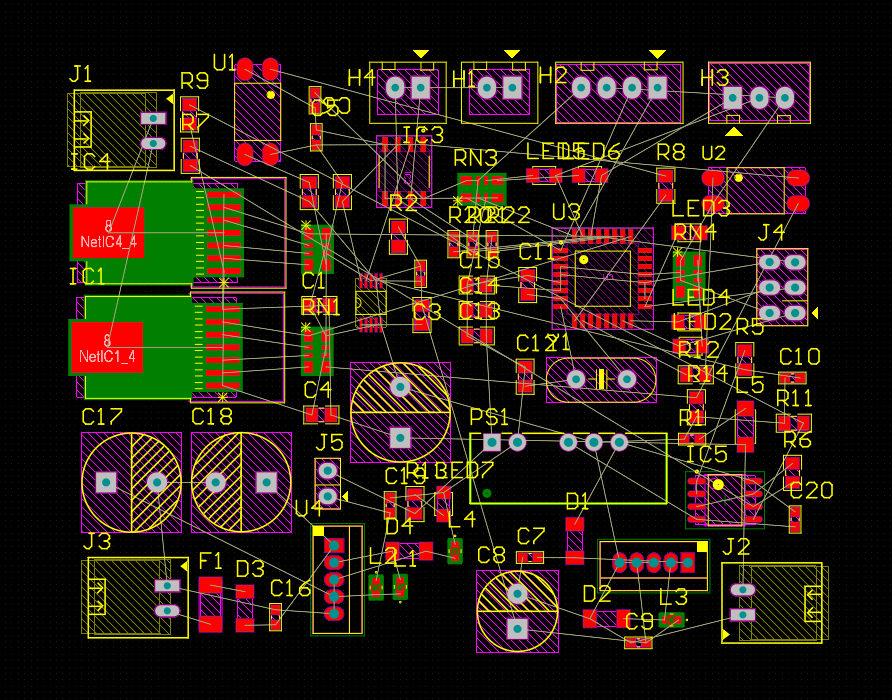
\includegraphics[width=0.8\textwidth]{pictures/7d.png}
\end{figure}
Khi sắp xếp vị trí linh kiện cần lưu ý sắp xếp làm sao để đường đi dây trên toàn mạch là ngắn nhất. Ngoài ra cần lưu ý khoảng cách giữa các linh kiện để không bị trùng lên nhay hoặc tồn tại quá nhiều khoảng trống không cần thiết.